\section{How to login to midway}

\subsection{ssh}
\begin{frame}[fragile]
  \frametitle{Login to midway: ssh}
  \begin{itemize}
  \item {\color{mycolorcli}ssh} - {\color{mycolordef}s}ecure {\color{mycolordef}sh}ell. 
  \item {\color{mycolordef}If you have an account on midway}:
{\color{mycolorcli}
\begin{verbatim}
ssh <cnetid>@midway2.rcc.uchicago.edu
\end{verbatim}
}
  \item This assumes that you have ssh client on your laptop.
  \item If you have Mac or run Linux on your laptop, you should have it
  \item If you have MS Windows, you might need to install a client: 
    for example {\color{mycolorcli}putty} or {\color{mycolorcli}bitvise} from  {\color{mycolorcli}\verb|http://www.putty.org|}.
  \item On Chromebook or any other OS you can use ssh extention to Chrome browser.
  \end{itemize}
\end{frame}

\subsection{yubikey}
\begin{frame}[fragile]
  \frametitle{Login to midway: yubikey}
  \begin{itemize}
  \item {\color{mycolordef}If you do not have an account on midway cluster}, use {\color{mycolordef}yubikey}:
    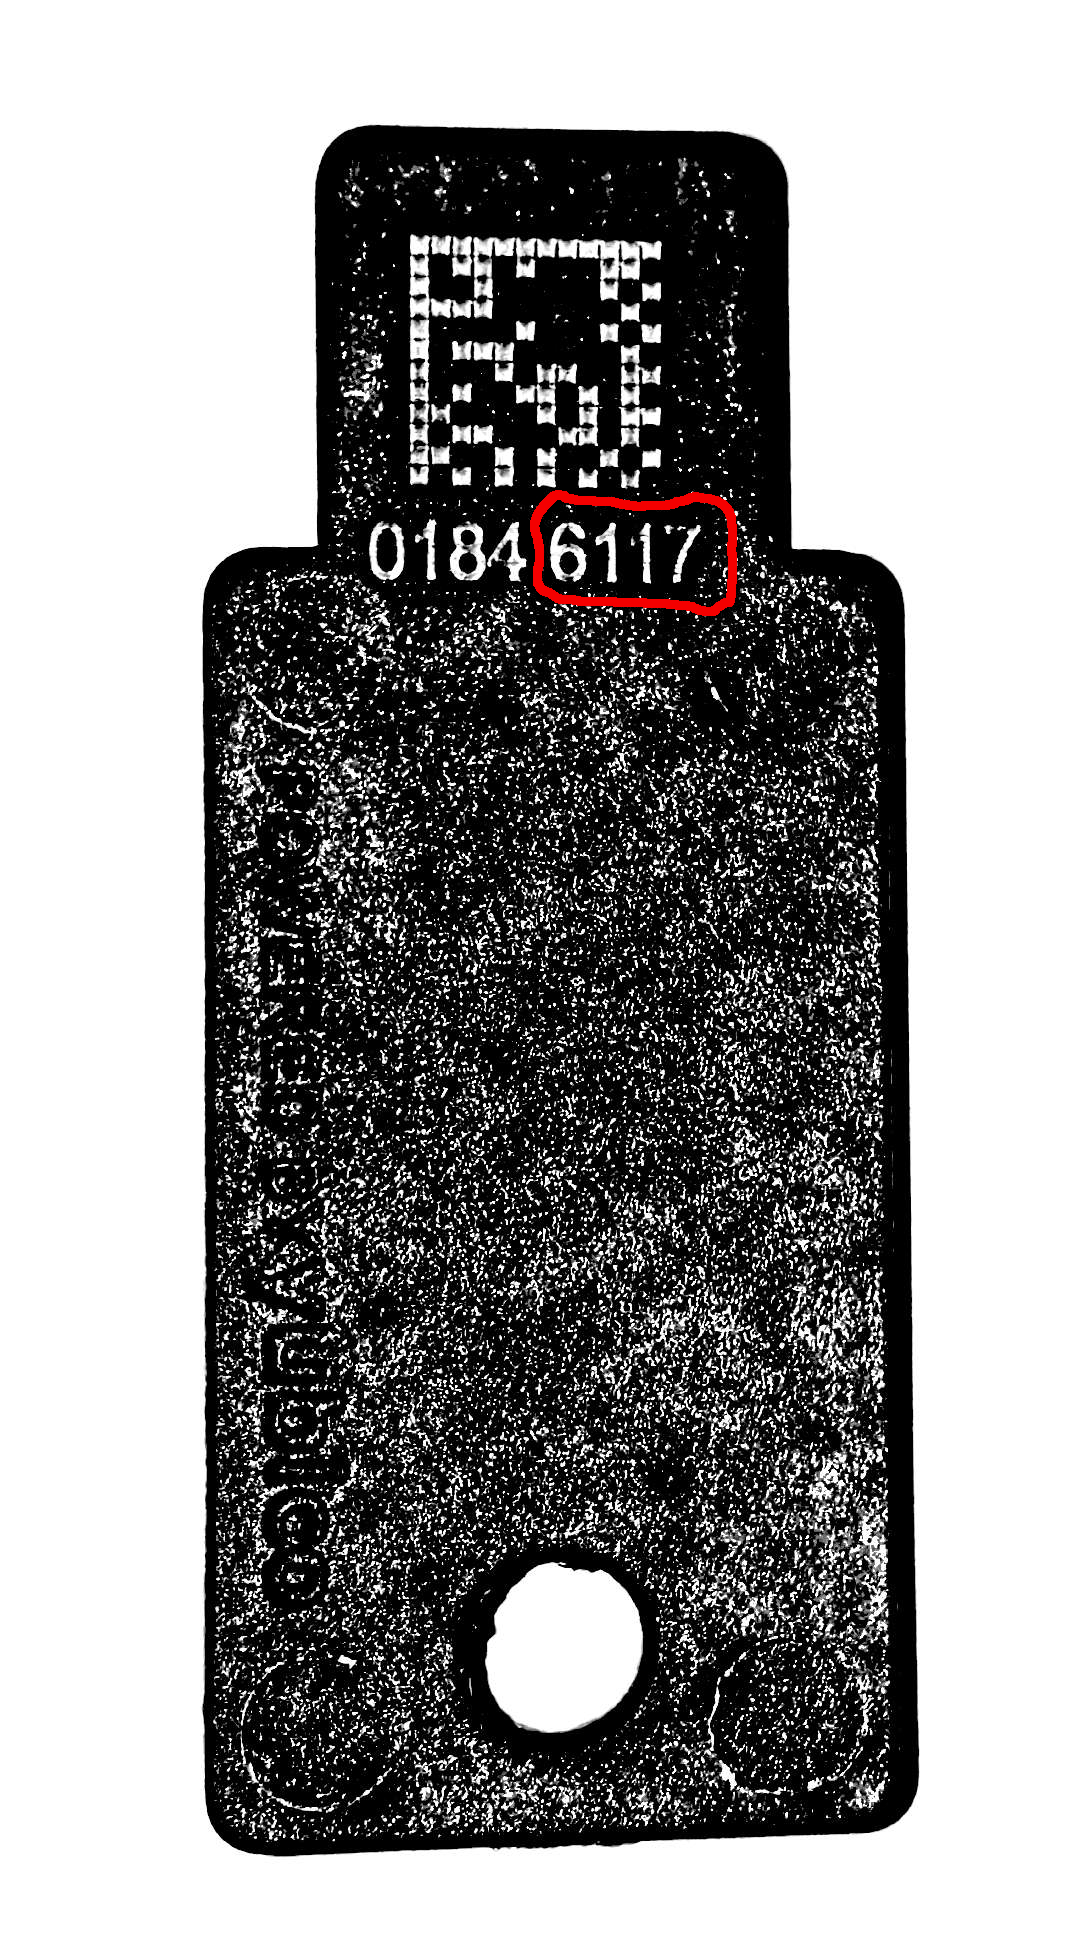
\includegraphics[width=1.5cm]{icons/yubikey1a.jpg}
    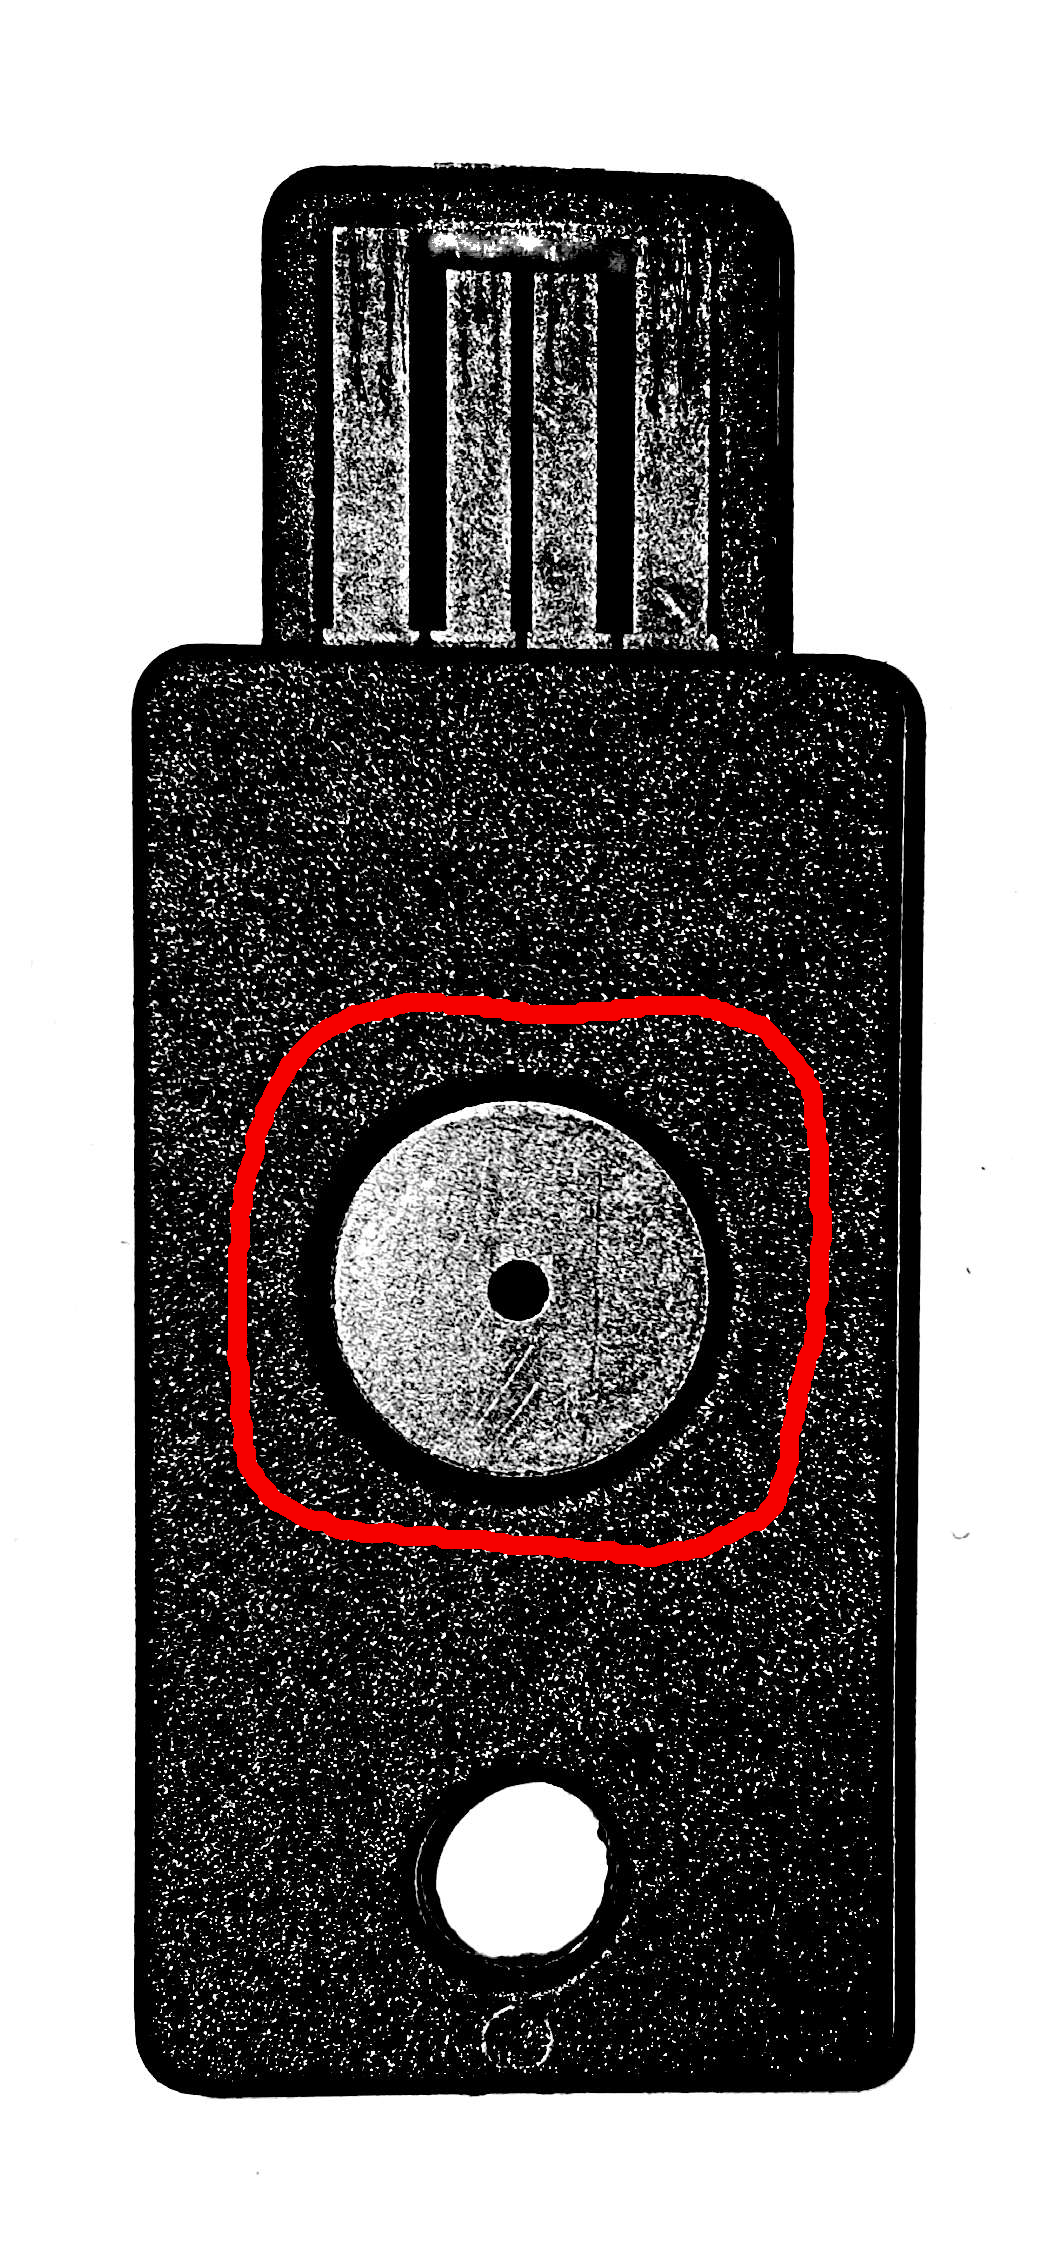
\includegraphics[width=1.3cm]{icons/yubikey2a.jpg}
    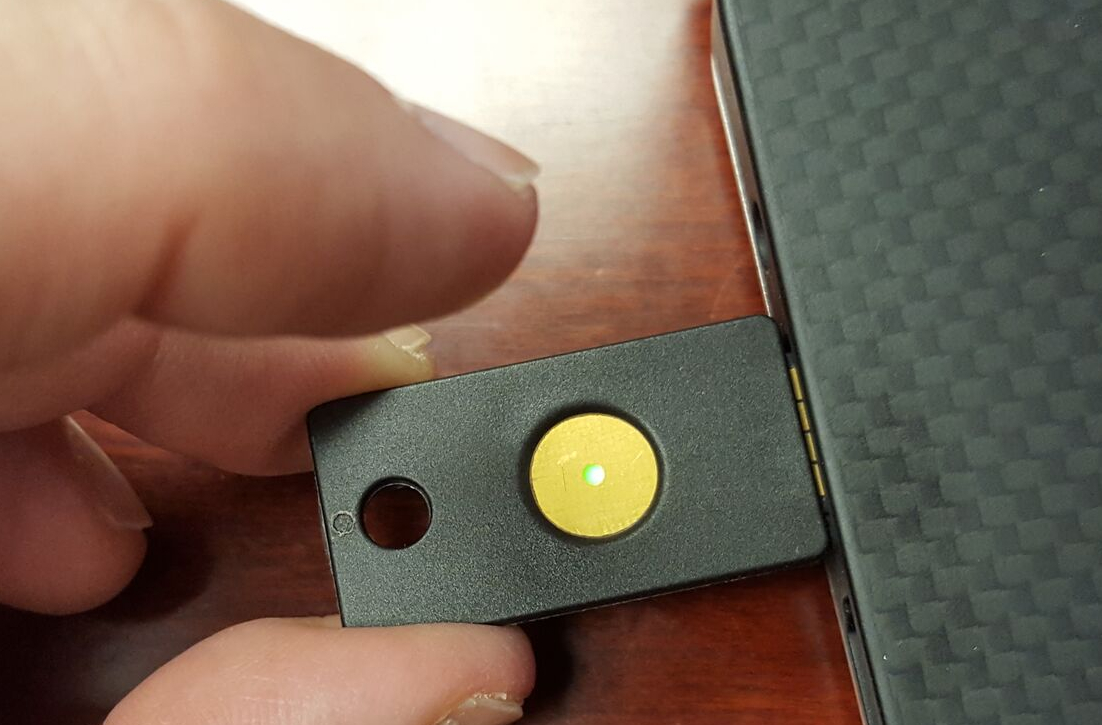
\includegraphics[width=3.3cm]{icons/yubikey3a.jpg}
  \item Use last 4 digits XXXX of yubikey as part of userid:
    {\color{mycolorcli}
\begin{verbatim}
ssh rccguest<XXXX>@midway2.rcc.uchicago.edu
\end{verbatim}
    }
  \item Push the button when asked for password
  \end{itemize}
\end{frame}

\subsection{ThinLinc}
\begin{frame}[fragile]
  \frametitle{Login to midway: ThinLinc}
  \begin{itemize}
    \item There are two ways to connect with ThinLinc to midway:
      \begin{itemize}
        \item Just use a web browser interface by pointing your browser to {\color{mycolorcli}\verb|https://midway2.rcc.uchicago.edu|}. 
          This might not work well for all browsers, you might have to try several: Chrome, Firefox, Safari...
        \item For Linux, Mac and Windows there is a client you can download from {\color{mycolorcli}\verb|https://www.cendio.com/thinlinc/download|}. 
          \begin{itemize}
          \item Configure the client to connect to {\color{mycolorcli}\verb|midway2.rcc.uchicago.edu|}
          \item You can specify the dimensions of the window in which it is running. I am usually using full screen.
          \end{itemize}
      \end{itemize}
    \item ThinLinc does not work with yubikeys, you need to have an account on midway
  \end{itemize}
\end{frame}
